\section{Considerações inicias}

A organização de uma coleção de documentos em vários tópicos, de modo que exista sobreposição entre
os grupos, é um importante problema em sistemas de recuperação de informação(SRIs). Na literatura,
diversas estratégias são utilizadas visando otimizar a organização flexível de documentos, conforme
foi abordado no capítulo anterior. Soma-se a isso o fato de que a maioria dos métodos que adicionam
flexibilidade ao processo, como por exemplo  os métodos de agrupamento, nem sempre são desenvolvidos
com o foco em documentos textuais, os quais possuem características que acrescentam algumas
dificuldades no processo, tais como a alta dimensionalidade dos dados, e o armazenamento de maneira
não estruturada \cite{Steinbach2004}.  Adicionalmente com o crescente aumento do uso de tecnologias
de produção de conteúdo, a quantidade de dados textuais tem alcançado grandes volumes de dados, o
que os enquadra no contexto do {\it Big Data\/}, fortalecendo a importância de se conduzir pesquisas
e investigações em torno da organização flexível de documentos. 

Nesse contexto, este capítulo tem como objetivo detalhar as contribuições desta monografia para
organização flexível de documentos, através da investigação dos impactos de se utilizar uma
estratégia híbrida de agrupamento fuzzy e possibilístico para a organização de documentos. Tal
estratégia dar-se-á pelo uso do algoritmo {\it Possibilistic Fuzzy C-Means\/}, o qual pretende
resolver os problemas dos elementos equidistantes e dos grupos coincidentes, apresentados nas
partições fuzzy e possibilística respectivamente. 

Conforme observa-se no capítulo 2, o algoritmo PFCM produz duas partições, sendo uma fuzzy e outra
possibilística, o que induziu o presente trabalho a propor duas extensões do método de extração de
descritores {\it Soft Organization - Fuzzy Description Comes Last\/} (SoftO-FDCL) proposto por
\citeonline{Nogueira2013}. O primeiro método proposto, denominado PDCL({\it Possibilistic Descriptor
Comes Last\/}), aborda uma nova estratégia de interpretação dos graus de compatibilidade da partição
possibilística.  Enquanto a segunda abordagem proposta,  Mixed-PFDCL({\it Mixed - Possibilistic
Fuzzy Descriptor Comes Last\/}), é uma adaptação do PDCL, utilizando uma abordagem híbrida para
mesclar as duas partições presentes no algoritmo PFCM. 

Nas seções a seguir são apresentadas informações das bases de dados utilizadas, com as
suas características, origem e composição dos documentos; um
estudo sobre a interpretação dos graus de compatibilidade possibilísticos durante a extração de
descritores; as propostas sugeridas por essa monografia, que derivam deste
estudo; e, por fim, os resultados obtidos com os experimentos realizados.

\section{Coleções textuais}
\label{section:datasets}

Na mineração de textos e consequentemente nos trabalhos relacionados à organização flexível de
documentos, é comum se realizar a avaliação dos métodos propostos, conduzindo-se experimentos sobre
coleções textuais existentes na literatura com essa finalidade \cite{Rossi2013}. Para isso, as
coleções precisam se estarem estruturadas. Assim sendo, nesta pesquisa foi adotada a estrutura de
representação de documentos textuais {\it tf-idf\/} apresentada no Capítulo \ref{ch:theory}, Equação
(\ref{eq:tfidf}), como forma de estruturar os dados presentes nas coleções, de modo a capturar a
importância relativa dos termos nos documentos e nas coleções, montando assim ao final do
pré-processamento uma matriz documentos x termos.

A base Opinosis\footnotemark é composta de opiniões de consumidores a respeito das características
de alguns produtos, obtidas dos portais amazon.com, tripadvisor e edmunds.com. As opiniões presentes
na base, abordam tópicos como serviços de hospedagem, dispositivos eletrônicos e carros. Sendo que
no total as sentenças presentes na coleção estão distribuídas em 51 categorias, onde cada categoria
possui 100 aproximadamente. Os dados dessa base foram obtidos no repositório {\it UCI Machine
Learning Repository\/} \cite{Frank2010}, que mantém várias coleções de dados que são utilizados pela
comunidade de aprendizado de máquina.
\footnotetext{\url{http://archive.ics.uci.edu/ml/datasets/Opinosis+Opinion+26frasl3B+Review}}

A coleção de documentos 20Newsgroup\footnotemark contém aproximadamente 20000 documentos de
\footnotetext{\url{http://qwone.com/~jason/20Newsgroups/}}
notícias, particionados em mais ou menos 20 temas. Para os experimentos realizados nesta pesquisa,
foi utilizado uma amostragem da coleção, contendo 2000 documentos pertencentes ao tema ciência, a
qual contém os tópicos sci.space, sci.electronics e sci.med. Esta base tem-se mostrado bastante
popular em aplicações textuais de aprendizado de máquina, tais como agrupamento e classificação de
textos.  Essa base foi coletada originalmente por Ken Lang para a pesquisa Newsweeder apresentada em
\cite{Lang1995}.  

Os documentos presentes na base de dados Reuters-21578\footnotemark  apareceram inicialmente na
\footnotetext{\url{https://archive.ics.uci.edu/ml/datasets/Reuters-21578+Text+Categorization+Collection}}
Reuters newswire em 1987. Sendo que os documentos foram coletados e indexados diretamente por
membros da Reuters e da {\it Carnegie Group, Inc.} também em 1987 para o desenvolvimento do
CONSTRUE \cite{Hayes1990}, que foi um sistema de categorização de documentos. No ano de 1990
essa base de dados foi tornada pública pela Reuters, para ser utilizada em pesquisas de recuperação
de informação. No entanto, as versões inicias dessa base continham documentos repetidos e ambíguos, o
que motivou um grupo de pesquisadores de categorização textual durante a conferência {\it ACM SIGIR
'96\/}, a realizar uma limpeza na base, possibilitando uma melhor comparação dos resultados entre
diferentes estudos. Essa versão final ficou com o total de 21578 documentos, distribuídos entre 43
diferentes categorias.  Nesta pesquisa foi utilizada uma amostragem da coleção
contendo 1052 documentos selecionados aleatoriamente de cada classe da coleção.

A base de dados WAP({\it WebACE Project\/}) é composta de um conjunto de páginas web coletadas por
\citeonline{Moore1997}, para um projeto de pesquisa de agrupamento, seleção e recuperação de páginas
web.  Os dados presentes nesta coleção foram obtidos pelos autores do artigo em 98 páginas web, onde
posteriormente foram distribuídos em 20 diferentes categorias, que abrangem tópicos como negócios e
finanças, tecnologias, trabalho e indústria. O conteúdo obtido está disposto em 1560 documentos na
sua versão original e todos os documentos foram utilizados nesta pesquisa.

A coleção de documentos NSF\footnotemark({\it National Science Foundation\/}) foi obtida do 
repositório de dados para pesquisas de aprendizado de máquina 
{\it UCI Machine Learning Repository} \cite{Frank2010}. O conteúdo dos dados presentes na base é
composto de 129000 resumos, sendo um resumo por documento, descrevendo prêmios da NSF para 
pesquisas básicas. Para os experimentos descritos nesta monografia, foram selecionados 1600 
documentos de maneira aleatória entre as categorias apresentadas na coleção.
\footnotetext{\url{https://archive.ics.uci.edu/ml/datasets/NSF+Research+Award+Abstracts+1990-2003}}

A base de dados Hitech adquirida em \citeonline{Karypis2006}, é parte de uma coleção de bases da
conferência TREC ({\it Text REtrieval Conference\/})\footnotemark.
\footnotetext{\url{http://trec.nist.gov/data.html}} Esta base é composta de um conjunto de notícias
da revista {\it Jose Mercury News\/}\footnotemark, as quais são distribuídas em categorias
\footnotetext{\url{http://www.mercurynews.com/}}
distintas. As notícias presentes na coleção abordam temas como computadores, eletrônicos, saúde,
medicina, pesquisa e tecnologia.  A base originalmente possui 2301 documentos e para esta pesquisa
foram selecionados 600 documentos aleatoriamente.  

Outro aspecto não menos importante, são as características particulares das coleções textuais. Pois
ressalta-se que para uma mais apurada análise dos resultados, é pertinente considerar as
particularidades de cada coleção, com a finalidade de encontrar possíveis justificativas para os
resultados apresentados, realizando-se indagações comparativas às peculiaridades sabidamente
conhecidas dos métodos analisados. O conjunto de características particulares de cada coleção 
obtidos em \citeonline{Rossi2013} e adaptados a esta pesquisa, dar-se à como apresentado
na Tabela \ref{table:datainfo}. 

\begin{table}[!htp]
  \centering
  \begin{tabular}{ |c|p{11cm}|}
    \hline
    {\bf documentos} & número de documentos presentes na coleção \\
    \hline
    {\bf termos} & número de termos existentes na coleção após o pré-processamento \\
    \hline
    {\bf \% zeros} & número relativo de zeros na {\it tf-idf\/}, quantificando o quanto a
matriz é esparsa \\
    \hline
    {\bf classes} & número de classes presentes na coleção \\
    \hline
    {\bf n-gramas} & quantidade de termos considerados sequencialmente na coleção \\
    \hline
  \end{tabular}
  \caption{Descrição das características objetivas presentes em coleções textuais elencadas para
este trabalho}
  \label{table:datainfo}
\end{table}

Uma análise objetiva das características presentes nas seis coleções utilizadas nos experimentos
pode ser observada na Tabela \ref{table:datasets}, onde é possível notar de maneira bem objetiva ao
se observar a coluna com o percentual de zeros da tabela, que todas as coleções apresentam uma
quantidade de zeros em mais de $90\%$ das frequências dos termos presentes na $tf-idf$, o que deixa
explícito o peculiar problema dos dados esparsos já caracterizado ao longo do texto, como algo
inerente aos dados textuais e que afeta negativamente grande parte dos resultados do processo de
mineração de textos.


\begin{table}[!htp]
  \centering
  \begin{tabular}{ |l|c c c c c|}
    \hline
    {\bf coleção} & {\bf docs} & {\bf termos} & {\bf classes} & {\bf \% zeros} & {\bf n-gramas} \\
    \hline
    {\bf Opinosis} & 51 & 842 & 3 & 95,73\% & 1-grama \\
    \hline
    {\bf 20newsgroups} & 2000 & 11028 & 4 & 99,11\% & 1-grama \\
    \hline
    {\bf Hitech} & 600 & 6925 & 6 & 97,93\% & 1-grama \\
    \hline
    {\bf NSF} & 1600 & 2806 & 16 & 99,76\% & 1-grama \\
    \hline
    {\bf WAP} & 1560 & 8070 & 20 & 98,51\% & 1-grama \\
    \hline
    {\bf Reuters-21578} & 1052 & 3925 & 43 & 98,55\% & 1-grama \\
    \hline
  \end{tabular}
  \caption{Características das coleções textuais utilizadas nesta pesquisa}
  \label{table:datasets}
\end{table}

A seguir, um refinamento organização flexível é abordado utilizando o algoritmo PFCM.

\section{Refinamento com o algoritmo PFCM}
\label{sec:exppfcm}

Conforme ficou evidenciado, a tarefa de organizar de maneira flexível um conjunto de documentos
textuais, possui diversos desafios. Em particular, ao se agrupar um conjunto de documentos é
esperado que os grupos resultantes possuam significado relevante, ou seja o algoritmo de
agrupamento precisa detectar a estrutura natural dos documentos \cite{Steinbach2004}. Alguns desses 
desafios estão na dificuldade em escalar os métodos usuais para coleções textuais na categoria {\it Very Large}
conforme a escala apresentada na Tabela \ref{table:datasize}; na obtenção de
mecanismos efetivos para se avaliar a qualidade dos grupos produzidos; nas técnicas para se medir a
interpretabilidade dos resultados; na capacidade para estimar os parâmetros dos algoritmos;
na possibilidade de funcionar de maneira incremental, reduzindo o custo computacional durante a
atualização dos grupos com novos dados; e, também na capacidade de continuar a produzir bons
resultados em cenários compostos de documentos ruidosos \cite{Carvalho2016}. 

Portanto, para \citeonline{Steinbach2004}:
\begin{citacao}
  {\it [...] there is no reason to expect that one type of clustering approach will
  be suitable for all types of data, even all high dimensional data. Statisticians and other
  data analysts are very cognizant of the need to apply different tools for different types of
  data, and clustering is no different\/}.
\end{citacao}

Diante dos desafios propostos, e com a evidência de que é possível aprimorar os resultados ao
se utilizar novas estratégias de agrupamento, a investigação apresentada nesta seção tem como
objetivo analisar de qual forma a organização de documentos pode ser otimizada, ao aplicar na etapa
de agrupamento uma estratégia que misture as partições possibilística e fuzzy, por meio do algoritmo
PFCM. 

Vale ressaltar, que a escolha desse algoritmo foi feita devido o seu potencial para absorver as
qualidades presentes no {\it Fuzzy C-Means\/} (FCM) contrabalanceando as suas deficiências ao
agregar também o {\it Possibilistic C-Means\/} (PCM) e sua partição possibilística. Além disso,
existem diversas pesquisas na literatura abordando o desempenho do PFCM, como por exemplo em
\citeonline{Pal2005,Yan2009,Kumar2010,Grover2014} e \citeonline{Popescu2015}.

Sendo assim, foram conduzidos experimentos adaptando a estratégia de organização flexível de documentos
definida em \citeonline{Nogueira2013},
utilizando na etapa de agrupamento o método PFCM. Uma vez que esse método produz duas partições, uma
possibilística e uma fuzzy, foi aplicado o método de extração de descritores
SoftO-FDCL na partição fuzzy e também na partição possibilística, produzindo assim dois grupos de
descritores. 

Com essa adaptação espera-se uma melhor organização dos documentos, de forma que melhores
descritores sejam escolhidos para caracterizar grupos. Tal processo de organização é ilustrado na
Figura \ref{fig:flexibleorganization}.

\begin{figure}[!htp] 
  \centering
  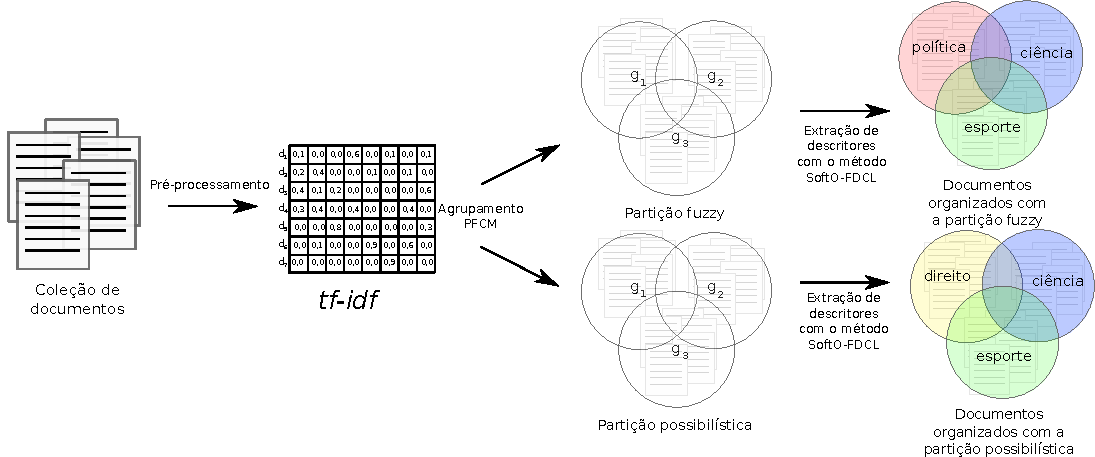
\includegraphics[width=1.0\columnwidth]{assets/process_pfcm.pdf} 
  \caption{Estratégia de organização flexível de documentos adotada ao se misturar abordagens fuzzy
  e possibilísticas no agrupamento} 
  \label{fig:flexibleorganization} 
\end{figure}

Para se calcular a quantidade ótima de grupos, para cada coleção foi utilizado o
método da silhueta fuzzy (Equação \ref{eq:fs}), método bastante utilizado com o propósito de avaliar
o agrupamento de documentos. Assim sendo, o número ideal de grupos é determinado após a execução da
silhueta fuzzy variando o número de grupos entre 2 e o número de classes de cada coleção.
Ressalta-se que em coleções que os documentos não possuem rótulos, ou seja o número de classes é
desconhecido, ainda é possível usar o método da silhueta fuzzy para definir o número ótimo de
grupos. No entanto, a quantidade máxima de grupos deve ser definida de modo empírico ou com base em
alguma informação prévia a respeito dos dados. 

Para permitir uma análise comparativa dos resultados, o experimento foi realizado também com os
algoritmos FCM e PCM.  Como resultado do agrupamento das coleções, está disposto na Tabela
\ref{table:pfcmclusters} a comparação do número de grupos obtidos por cada algoritmo de agrupamento.
Nessa comparação nota-se que os algoritmos FCM e PFCM foram os que alcançaram uma quantidade de
partições mais próxima da quantidade de classes existentes em cada coleção. Enquanto o PCM manteve
uma tendência a produzir uma quantidade menor de grupos em relação aos demais.

\begin{table}[!htp]
  \centering
  \begin{tabular}{ |l|c|c|c|c|}
    \hline
    {\bf coleção} & {\bf \# classes} & {\bf FCM} & {\bf PCM} & {\bf PFCM} \\
    \hline
    Opinosis & 3 & 3 & 3 & 3 \\
    \hline
    20Newsgroup & 4 & 2 & 2 & 2 \\
    \hline
    Hitech & 6 & 6 & 5 & 5 \\
    \hline
    NSF & 16 & 11 & 2 & 16 \\
    \hline
    WAP & 20 & 14 & 5 & 16 \\
    \hline
    Reuters-21578 & 43 & 22 & 11 & 36 \\
    \hline
  \end{tabular}
  \caption{Quantidade ótima de grupos determinada através do método da silhueta fuzzy para cada
  algoritmo de agrupamento}
  \label{table:pfcmclusters}
\end{table}

Após agrupar os dados utilizando os métodos FCM, PCM e PFCM, foi aplicado o método de extração 
de descritores SoftO-FDCL. Para avaliar os descritores produzidos, foi verificado o
potencial preditivo dos mesmos, possibilitando assim quantificar a qualidade dos
termos selecionados para nomear os grupos. 

A avaliação do potencial preditivo dos descritores foi realizada, realizando se uma defuzificação
dos grupos produzidos pelo agrupamento, ou seja, se durante o agrupamento foi gerado o conjunto
de grupos $G = \{g_1,g_2,...,g_c\}$, temos então o conjunto de grupos $crisp$ $C' =
\{crisp_1,crisp_2,...,crisp_c\}$, onde cada $crisp_i$ corresponde ao grupo $g_i$. A função de
defuzificação adotada para se converter as
as partições fuzzy e possibilística, as quais permitem que um documento pertença a um ou mais
grupos, considera o grupo $crisp$ de um documento $d_i$, como sendo o grupo $crisp_j$ do respectivo
$grupo_j$, no qual $d_i$ possui a maior
pertinência/tipicidade. Esta definição está formalizada na Equação (\ref{eq:class}).

\begin{equation}
  crisp(d_i) = \begin{cases}
    crisp_j, & \mu(d_i,g_j) = \displaystyle\max_{\forall g \in G} \mu(d_i,g), \text{se a partição
  for fuzzy}\\
  crisp_j, & \lambda(d_i,g_j) = \displaystyle\max_{\forall g \in G} \lambda(d_i,g), \text{se a
  partição for possibilística}
  \end{cases}
  \label{eq:class}
\end{equation}

Após se atribuir os documentos aos grupos $crisp$, é produzida uma outra matriz,
considerando apenas os termos descritores dos grupos. Logo, essa matriz documentos x descritores
$D'_{n \times m}$, 
é uma versão condensada da matriz documentos x termos $D_{n \times k}$, onde $n$ corresponde a 
quantidade de documentos, $k$ à quantidade de termos e $m$ à quantidade de descritores. O conteúdo
dessa matriz condensada, assim como na matriz original, é a frequência dos descritores nos 
documentos. 

Visando avaliar a qualidade dos descritores e permitir uma comparação direta dos impactos
dessa abordagem com os resultados publicados em \citeonline{Nogueira2013} e
\citeonline{Nogueira2015}. Submeteu-se a matriz $D'$ 
aos algoritmos de classificação 
SVM, Naive Bayes, Multinomial Naive Bayes, KNN e C4.5, que são bem comuns na avaliação de 
métodos de aprendizado de máquina, e foram os mesmos utilizados em \citeonline{Nogueira2015}.

Nesse contexto, foi utilizada a implementação dos algoritmos de classificação anteriormente citados
presentes na ferramenta WEKA \cite{weka}. Os algoritmos Naive Bayes (NB), Multinomial Naive Bayes
(NB-Multinomial) e o J48 (que é a implementação do C4.5 existente no WEKA), foram executados com os
parâmetros padrão da ferramenta. Por outro lado, o SVM foi ajustado para usar o {\it Normalized
Polynomial Kernel\/} com o parâmetro de complexidade sendo $c = 2.0$. O algoritmo IBk (implementação
do KNN presente no WEKA) foi executado 7 vezes, variando o parâmetro de vizinhos de 1 até 7, sendo
escolhido o melhor resultado. Ressalta-se que foi adotada a técnica {\it 10-fold cross validation\/}
no experimento para melhor capturar a capacidade de generalização do modelo. Os resultados dessa
avaliação estão apresentados nas Figuras \ref{fig:pfcmopinosis},  \ref{fig:pfcm20news},
\ref{fig:pfcmhitech}, \ref{fig:pfcmnsf}, \ref{fig:pfcmwap} e \ref{fig:pfcmreuters}. 

\begin{figure}[!htp] \centering 
   \begin{minipage}{0.45\textwidth} 
     \centering
    \includegraphics[width=1.0\columnwidth]{assets/pfcm/opinosis} 
    \caption{Desempenho obtido com os descritores extraídos com o algoritmo SoftO-FDCL a partir dos
      métodos de agrupamento FCM,
    PCM e PFCM executados na coleção Opinosis} 
  \label{fig:pfcmopinosis}
  \end{minipage}\hfill 
  \begin{minipage}{0.45\textwidth} \centering
    \includegraphics[width=1.0\columnwidth]{assets/pfcm/newsgroup} 
    \caption{Desempenho obtido com os descritores extraídos com o algoritmo SoftO-FDCL a partir dos
      métodos de agrupamento FCM,
    PCM e PFCM executados na coleção 20Newsgroup} 
     \label{fig:pfcm20news} 
   \end{minipage} 
\end{figure}

\begin{figure}[!htp] \centering 
   \begin{minipage}{0.45\textwidth} 
     \centering
    \includegraphics[width=1.0\columnwidth]{assets/pfcm/hitech} 
    \caption{Desempenho obtido com os descritores extraídos com o algoritmo SoftO-FDCL a partir dos
      métodos de agrupamento FCM,
    PCM e PFCM executados na coleção Hitech} 
  \label{fig:pfcmhitech}
  \end{minipage}\hfill 
  \begin{minipage}{0.45\textwidth} \centering
    \includegraphics[width=1.0\columnwidth]{assets/pfcm/nsf} 
    \caption{Desempenho obtido com os descritores extraídos com o algoritmo SoftO-FDCL a partir dos
      métodos de agrupamento FCM,
    PCM e PFCM executados na coleção NSF} 
     \label{fig:pfcmnsf} 
   \end{minipage} 
\end{figure}

\begin{figure}[!htp] \centering 
   \begin{minipage}{0.45\textwidth} 
     \centering
    \includegraphics[width=1.0\columnwidth]{assets/pfcm/wap} 
    \caption{Desempenho obtido com os descritores extraídos com o algoritmo SoftO-FDCL a partir dos
      métodos de agrupamento FCM,
    PCM e PFCM executados na coleção WAP} 
    \label{fig:pfcmwap}
  \end{minipage}\hfill 
  \begin{minipage}{0.45\textwidth} \centering
    \includegraphics[width=1.0\columnwidth]{assets/pfcm/reuters} 
    \caption{Desempenho obtido com os descritores extraídos com o algoritmo SoftO-FDCL a partir dos
      métodos de agrupamento FCM,
    PCM e PFCM executados na coleção Reuters-21578} 
     \label{fig:pfcmreuters} 
   \end{minipage} 
\end{figure}

O resumo dos resultados do desempenho dos descritores extraídos após o agrupamento com os
algoritmos FCM, PCM e PFCM é apresentado na Tabela \ref{table:pfcmsummary}. Na tabela, a marcação
($\checkmark$) denota qual método de agrupamento obteve a maior taxa de classificação dentre os
demais.

\begin{table}[!htp]
  \centering
  \begin{tabular}{ |l|c c c c c c c|}
    \hline
    {\bf nome} & docs & termos & classes & \% zeros & FCM & PCM & PFCM \\
    \hline
    {\bf Opinosis} & 51 & 842 & 3 & 95,73\% & & $\checkmark$ &  \\
    \hline
    {\bf 20newsgroups} & 2000 & 11028 & 4 & 99,11\% & & & $\checkmark$\\
    \hline
    {\bf Hitech} & 600 & 6925 & 6 & 97,93\% & $\checkmark$ & & \\
    \hline
    {\bf NSF} & 1600 & 2806 & 16 & 99,76\% & $\checkmark$ & & \\
    \hline
    {\bf WAP} & 1560 & 8070 & 20 & 98,51\% & & & $\checkmark$ \\
    \hline
    {\bf Reuters-21578} & 1052 & 3925 & 43 & 98,55\% & $\checkmark$ & & \\
    \hline
  \end{tabular}
  \caption{Sumário dos resultados da classificação dos descritores}
  \label{table:pfcmsummary}
\end{table}

Esses resultados obtidos reforçam a flexibilidade e adaptação do método SoftO-FDCL
\cite{Nogueira2013}, a novos algoritmos de agrupamento, demonstrando-se promissor na tarefa de
extrair termos relevantes dos grupos produzidos na etapa de agrupamento. Tal expectativa é
demonstrada por meio do potencial preditivo evidenciado na Tabela \ref{table:pfcmsummary}, com as
taxas máximas de classificação de mais de 80\% para quase todas as coleções, com exceção da base
Hitech, a qual obteve a taxa máxima de 58.67\%.  

Adicionalmente, ressalta-se a importância também de avaliar de maneira subjetiva os descritores
selecionados dos grupos, permitindo  compreender se os termos obtidos fazem sentido para a
organização de documentos em grupos. 

\begin{table}[!htp]
  \centering
  \begin{tabular}{ |l|p{4cm} | p{4cm} | p{4cm}|}
    \hline
    {\bf método} & $crisp_1$ & $crisp_2$ & $crisp_3$ \\
    \hline
    {\bf FCM} & easy, clear, drive, display, control, car, version, nice, work, perfect & fact,
    import, isn't, model, problem, unit, design, don't, doesn't, found & breakfast, nearby,
    concierge, eat, bottle, coffee, floor, food, inn, friendly \\
    \hline
    {\bf PCM} & easy, read, problem, version, don't, small, nice, car, work, found & fact, back,
    turn, expect, size, close, quality, review, min, feature & feel, amazing, isn't, extreme, drive,
    include, point, reason, give, run\\
    \hline
    {\bf PFCM $\mu$} & easy, drive, control, don't, version, nice, car, work, perfect, lot & fact,
    isn't, read, complete, device, display, size, doesn't, found & breakfast, nearby, pleasant,
    concierge, eat, coffee, floor, clean, friendly, food\\
    \hline
    {\bf PFCM $\lambda$} & club, immaculate, send, towel, basic, exception, spotl, pillow, typical,
    fridge & pub, housekeep, holiday, tourist, tea, smoke, pm, renovate, facilite, london & usual,
    central, forum, bottle, modern, adult, supply, food, reserve, dinner\\
    \hline
  \end{tabular}
  \caption{Descritores extraídos com os métodos de agrupamento FCM, PCM e PFCM da coleção Opinosis,
  onde $\mu$ e $\lambda$ se referem as partições fuzzy e possibilística respectivamente, da qual os
descritores foram extraídos.}
  \label{table:pfcmdescriptors}
\end{table}

Sendo assim, para uma análise subjetiva dos resultados, os descritores da coleção Opinosis, foram
obtidos por possuir poucos grupos e assim facilitar a análise e a visualização. A coleção Opinosis
contém opiniões dos usuários a respeito de serviços de hospedagem, dispositivos eletrônicos e carros
e espera-se que os descritores de grupos se aproximem semanticamente de tais categorias.  Na Tabela
\ref{table:pfcmdescriptors} tem-se a seleção de descritores escolhidos para cada grupo, extraídos
pelos algoritmos FCM, PCM e PFCM. Ao analisar os descritores selecionados é possível notar uma
tendência geral, do grupo $crisp_1$ conter descritores relacionadas a carros, o $crisp_2$ conter
descritores sobre dispositivos eletrônicos e o grupo $crisp_3$ descritores sobre hospedagem e
alimentação. Contudo, nota-se que os descritores do PCM e do PFCM$\lambda$ (descritores da partição
possibilística do PFCM) estão um pouco mais misturados, não apresentando uma tendência geral bem
definida. Uma explicação possível a esse resultado pode se encontrar na própria partição
possibilística a qual permite que um mesmo documento possua um grau de tipicidade elevado em todos
os grupos. Neste contexto, uma solução possível pode ser uma adaptação do método de extração de
descritores SoftO-FDCL voltado para a partição possibilística, assim como também para algoritmos
híbridos com duas partições, que é o caso do PFCM.

De maneira complementar, é importante salientar que o método de extração de descritores SoftO-FDCL é
totalmente influenciado pelos valores contidos nas partições fuzzy e possibilística. Portanto, é
também importante realizar uma análise dos métodos de agrupamento utilizados nos experimentos, com
a finalidade de entender qual método é mais apropriado em determinados contextos. Os resultados apontam que a dimensionalidade das bases foi um fator determinante no desempenho dos
métodos de agrupamento para a organização flexível de documentos, e, consequentemente, a
extração de descritores. Por exemplo, do sumário de resultados apresentados na Tabela
\ref{table:pfcmsummary}, é possível observar que o método PCM obteve o melhor resultado na coleção
Opinosis, que possui a menor dimensionalidade (842 termos), enquanto que o algoritmo FCM superou os
demais métodos na coleção NSF (2806 termos), Reuters-21578 (3925 termos), Hitech (6925 termos), e por
fim o algoritmo PFCM atingiu melhores resultados para as coleções WAP (8070 termos) e 20Newsgroup
(11028 termos), que são as coleções de maior dimensionalidade.

Na próxima seção, motivado pelos resultados desses experimentos será explorado, uma adaptação do
método SoftO-FDCL para evitar o processo de extração dupla de descritores em algoritmos que possuam
partições fuzzy e possibilística.

\section{Uma abordagem híbrida para extração de descritores}

Nos experimentos anteriores foi identificado um possível problema ao realizar a extração dos
descritores de maneira separada em cada partição do PFCM, assim como também foi apontado que o
método pode não capturar toda essência da partição possibilística, que difere da partição fuzzy do
FCM por não possuir a restrição que obriga a soma das pertinências de um grupo ser igual a um
(Equação \ref{eq:fcmrestri1}).
Logo, é intuitivo indagar que para uma melhor interpretação dos grupos produzidos em um método de
agrupamento híbrido, seja pertinente utilizar também uma abordagem mista de extração de descritores.
Aproveitando-se assim dos benefícios existentes na partição possibilística, a qual penaliza os
elementos ruidosos, com baixos valores de tipicidade, sem abrir mão das vantagens presentes na
partição fuzzy. Para isso é necessário compreender os mecanismos de funcionamento do método
SoftO-FDCL, para que seja possível propor uma adaptação para este contexto.

\subsection{Investigações na extração de descritores em partições possibilísticas}
\label{sec:softofdcl}

O método SoftO-FDCL ({\it Soft Organization - Fuzzy Description Comes Last}) proposto em 
\citeonline{Nogueira2013} é baseado em uma adaptação das medidas clássicas de Recuperação de
Informação (RI), para quantificar a relevância dos termos candidatos à descritores dos grupos
obtidos na etapa de agrupamento, utilizando a informação de pertinência ou tipicidade advinda do
algoritmo de agrupamento.  Esse grau de compatibilidade entre um documento e um grupo, desempenha um
papel fundamental na seleção dos termos candidatos a descritores de um determinado grupo, pois
através deste, é possível penalizar os termos de documentos que possuam baixo grau de
compatibilidade com o grupo no qual o descritor está sendo extraído.  

Para realizar a extração dos descritores, inicialmente todos os termos que permanecem na coleção
após a etapa de pré-processamento são considerados como candidatos a descritores. Posteriormente o
método realiza uma avaliação quantitativa da relevância de cada termo $t_k$ para um grupo $g_j$,
utilizando a medida $f1$ apresentada na Equação \ref{eq:fmeasure}, que é a média harmônica da
precisão (Equação \ref{eq:precision}) e da revocação (Equação \ref{eq:recall}).  A medida de
precisão checa a quantidade de documentos significantes entre os documentos recuperados. Enquanto a
medida de revocação calcula a proporção de documentos relevantes recuperados entre todos os
documentos relevantes da coleção. Tanto a medida de precisão quanto a de revocação, tomam como base
as informações obtidas a partir da matriz de contingência apresentada na Tabela
\ref{table:softmatrix}. Adicionalmente tem-se que um documento $d_i$ é considerado como parte do
grupo $g_j$, caso $\mu(d_j,g_j) \geq \delta$ para valores de pertinências ou $\lambda(d_i,g_j) \geq
\delta$ para partição possibilística, onde $\delta = \frac{1}{c}$ e $c$ a quantidade de grupos. O
limiar $\delta$ é uma parte relevante do método SoftO-FDCL, pois ele possibilita considerar como
candidatos a descritores, os termos presentes em documentos que pertençam a mais de um grupo, ao
mesmo tempo que também penaliza os termos presentes em documentos com baixa compatibilidade em um
grupo.

\begin{table}[!htp]
  \centering
  \begin{tabular}{ |p{5cm}|p{5cm}|p{5cm}|}
    \cline{2-3}
    \multicolumn{1}{p{5cm}|}{} & Documentos do grupo $g_j$ com grau de compatibilidade 
    maior ou igual a $\delta$ &
    Documentos do grupo $g_j$ com grau de compatibilidade menor do que $\delta$ \\
    \hline
    Documentos que possuem o descritor candidato $t_k$ & \parbox[c]{5cm}{\centering $ganhos$} &
    \parbox[c]{5cm}{\centering \it ruídos\/} \\
    \hline
    Documentos que não possuem o descritor candidato $t_k$ & \parbox[c]{5cm}{\centering $perdas$} &
    \parbox[c]{5cm}{\centering $rejeitos$} \\
    \hline
  \end{tabular}
  \caption{Matriz de contingência do termo $t_k$ para o grupo $g_j$ para as medidas de recuperação
  de informação}
  \label{table:softmatrix}
\end{table}

\begin{equation}
  precis\tilde{a}o(t_k,g_j) = \frac{ganhos}{ganhos + \text{\it ruídos}}
  \label{eq:precision}
\end{equation}
\begin{equation}
  \text{\it recuperação\/}(t_k,g_j) = \frac{ganhos}{ganhos + perdas}
  \label{eq:recall}
\end{equation}
\begin{equation}
  f1(t_k,g_j) = \frac{2 * \text{\it precisão}(t_k,g_j) * \text{\it recuperação}(t_k,g_j)}
  {\text{\it precisão}(t_k,g_j) + \text{\it recuperação}(t_k,g_j)}
  \label{eq:fmeasure}
\end{equation}

Para efetuar a seleção dos termos descritores, é construído um $ranking$ dos termos candidatos de
cada grupo, ordenados pela pontuação obtida com a medida $f1$ (Equação \ref{eq:fmeasure}). A partir
dessa pontuação, os termos com as maiores pontuações em cada grupo são selecionados.
\citeonline{Nogueira2013} destaca que a quantidade de descritores a ser selecionada fica a critério
do usuário.

Em síntese, o método SoftO-FDCL cria uma tabela de pontuação dos termos candidatos aos grupos,
e seleciona os que obtiverem melhores valores de $f1$.  

Formalizando essa
percepção, é possível definir as duas propriedades que derivam dessa discussão, as quais são as
Equações (\ref{eq:limiarp1}) e (\ref{eq:limiarp2}). A primeira
propriedade  apresentada na Equação (\ref{eq:limiarp1}) expressa que se um documento possuir pertinência maior do
que o limiar $\delta$ em um grupo $g_1$ qualquer, obrigatoriamente existirá ao menos um outro grupo
$g_2$ no qual esse mesmo documento terá pertinência inferior ao limiar $\delta$. Portanto, essa
propriedade nos indica que na maioria das vezes um ou mais documentos serão descartados na análise
dos termos candidatos do grupo, o que reforça a adequação desse limiar para a partição de
pertinências. Por outro lado, a segunda
propriedade apresentada na Equação (\ref{eq:limiarp2}) denota o único caso particular, no qual um documento $d_i$
não será descartado em nenhum grupo. Isto ocorre apenas se $d_i$ possuir pertinência igual ao limiar em todos
os grupos, o que só acontece em dados ruidosos, que apresentam o problema do elemento equidistante
detalhado na Figura \ref{fig:fcm_problem} do Capítulo 2.

\begin{equation}
  \mu(d_1,g_1) > \delta \rightarrow \exists \mu(d_i, g_2) < \delta
  \label{eq:limiarp1}
\end{equation}
\begin{equation}
  ( \mu(d_1,g_1) = \delta ) \wedge ( \mu(d_i,g_2) = \delta ) \wedge ... \wedge ( \mu(d_i,g_{c-1}) =
  \delta ) \rightarrow ( \mu(d_i, g_c) = \delta  )
  \label{eq:limiarp2}
\end{equation}

Contudo, para a partição possibilística, essas duas propriedades não são satisfeitas. Isso ocorre
devido a remoção da restrição da Equação (\ref{eq:fcmrestri1}), o que permite o grau de
compatibilidade da partição possibilística variar de maneira independente entre o intervalo de
$[0,1]$, sem ser influenciado pelo grau de compatibilidade do documento nos demais grupos.

Para tornar claro essas análises, considere uma situação onde tem-se uma coleção de textos com
3 documentos (Tabela \ref{table:sampledocuments}), onde cada documento possui 3 termos. Essa coleção
de documentos foi agrupada, usando o método PFCM, o qual produziu 2 grupos, com as suas
respectivas partições de pertinência (Tabela
\ref{table:samplefcmclusters}) e possibilística (Tabela \ref{table:samplepcmclusters}).

\begin{table}[!htp]
  \centering
  \begin{tabular}{ |c|c|c|c|}
    \hline
    & $\mathbfit{t_1}$ & $\mathbfit{t_2}$ & $\mathbfit{t_3}$ \\
    \hline
    $\mathbfit{d_1}$ & 0 & 0 & 1 \\
    \hline
    $\mathbfit{d_2}$ & 1 & 1 & 0 \\
    \hline
    $\mathbfit{d_2}$ & 1 & 1 & 0 \\
    \hline
  \end{tabular}
  \caption{Exemplo de matriz documentos x termos}
  \label{table:sampledocuments}
\end{table}

\begin{table}[!htp]
  \begin{minipage}{0.45\textwidth} 
    \centering
    \begin{tabular}{ |c|c|c|}
      \hline
      & $\mathbfit{g_1}$ & $\mathbfit{g_2}$ \\
      \hline
      $\mathbfit{d_1}$ & 0.5 & 0.5 \\
      \hline
      $\mathbfit{d_2}$ & 0.3 & 0.7 \\
      \hline
      $\mathbfit{d_3}$ & 0.3 & 0.7 \\
      \hline
    \end{tabular}
    \caption{Exemplo de matriz documents x grupos com graus de pertinência}
    \label{table:samplefcmclusters}
  \end{minipage}\hfill 
  \begin{minipage}{0.45\textwidth} 
    \centering
    \begin{tabular}{ |c|c|c|}
      \hline
      & $\mathbfit{g_1}$ & $\mathbfit{g_2}$ \\
      \hline
      $\mathbfit{d_1}$ & 0.7 & 0.7 \\
      \hline
      $\mathbfit{d_2}$ & 0.5 & 0.8 \\
      \hline
      $\mathbfit{d_3}$ & 0.5 & 0.9 \\
      \hline
    \end{tabular}
    \caption{Exemplo de matriz documents x grupos com graus de possibilidade}
    \label{table:samplepcmclusters}
  \end{minipage}\hfill 
\end{table}

A partir desse agrupamento é possível aplicar a extração de descritores, utilizando as partições
apresentadas nas Tabelas \ref{table:samplefcmclusters} e \ref{table:samplepcmclusters}. Seguindo
o procedimento do método SoftO-FDCL, inicialmente devemos considerar todos os descritores
presentes na Tabela \ref{table:sampledocuments}, como candidatos a descritores. Então, para
promover os descritores candidatos do grupo $g_1$ utilizando os graus de pertinências, deve-se 
observar os documentos que possuem pertinência maior ou igual ao limiar, onde no exemplo é
igual a $\delta = \frac{1}{2} = 0.5$. Portanto, o único documento que se enquadra no filtro do limiar
é o documento $d_1$ e o termo $t_3$, que é o único presente no documento $d_1$, é promovido
a descritor candidato e consequentemente a descritor do grupo $g_1$. Já o grupo $g_2$ possui 3
documentos com pertinência maior ou igual ao limiar $\delta$. Sendo assim, os termos de $d_1,d_2$ e
$d_3$ são promovidas a descritores candidatos do grupo $g_2$. Ao calcular-se a medida $f1$ para cada
um deles temos: $f1(t_1,g_2) = 0,8$, $f1(t_2,g_2) = 0,8$, $f1(t_3,g_2) = 0,5$. Logo, os descritores
selecionados para cada grupo foram $g_1 =\{t_3\}$ e $g_2 = \{t_1, t_2\}$.

Ao aplicar a extração de descritores sobre a partição possibilística, tem-se agora
os documentos $d_1, d_2$ e $d_3$ considerados parte do grupo $g_1$, de acordo com a regra do
limiar. Logo, deve-se considerar os termos dos 3 documentos como descritores candidatos. Os valores
de $f1$ para os 3 termos candidatos do grupo $g_1$ são: $f1(t_1,g_1) = 0,8$,
$f1(t_2,g_1) = 0,8$, $f1(t_3,g_1) = 0,5$. Para o grupo $g_2$ obtém-se os mesmos termos
candidatos, pois $d_1, d_2$ e $d_3$ também possuem valores de tipicidade maiores ou igual ao limiar
$\delta$, portanto os valores de $f1$ para o grupo $g_2$ são:  $g_1$: $f1(t_1,g_1) = 0,8$,
$f1(t_2,g_1) = 0,8$, $f1(t_3,g_2) = 0,5$. Foi obtido a mesma pontuação para os mesmos termos
candidatos nos dois grupos. Com isso, fica claro as causas que levaram a extração dos descritores
confusos apresentados na Tabela \ref{table:pfcmdescriptors}.  Ao se utilizar a mesma intepretação
dos graus de pertinência do FCM, nas tipicidades, o critério chave de descarte dos documentos de
baixa relevância em um grupo deixou de fazer efeito.

É importante ressaltar que esta situação se agrava ainda mais com o aumento do número de grupos
produzidos pelo agrupamento, pois quanto maior for a quantidade de grupos, menor será o valor do
limiar $\delta$. Esta noção fica explícita na terceira propriedade do limiar apresentada na Equação
(\ref{eq:limiarp3}). Ou seja, mais facilmente os graus de compatibilidade possibilísticos irão
passar no filtro do limiar, e, consequentemente todos os documentos serão considerados relevantes
para todos os grupos. 

\begin{equation}
  \lim_{c \rightarrow \infty} \delta = 0
  \label{eq:limiarp3}
\end{equation}


Na próxima seção será descrito uma possível proposta para interpretação dos graus de compatibilidade
das partições possibilística.

\subsection{Interpretando os graus de compatibilidade das partições possibilísticas}

A interpretação direta dos graus de compatibilidade possibilísticos gera uma série de problemas na
extração de descritores, conforme ficou demonstrado na seção anterior. Com isso, podemos formular a
seguinte pergunta: Como interpretar corretamente os graus de compatibilidade possibilísticos para
corretamente identificar os documentos relevantes de um dado grupo? Sabe-se que o valor de
tipicidade pode variar livremente entre o intervalo $[0,1]$, sem a restrição probabilística
(Equação \ref{eq:fcmrestri1}) do FCM. Essa é uma
característica positiva introduzida em \citeonline{Krishnapuram1993}, a qual atribui valores de
pertinência mais justos aos grupos fuzzy, em consonância com a teoria de conjuntos fuzzy proposta em
\citeonline{Zadeh1965} e brevemente contextualizada no Capítulo 2. Para melhor compreendermos esse
conceito de valores mais justos, podemos analisar o que os autores defenderam na publicação
original:

\begin{citacao}
Since our membership functions correspond more closely to
the notion of typicality, the resulting algorithms are naturally
more immune to noise. Noise points will have low degrees
of compatibility in all clusters, which makes their effect on
the clustering negligible \cite{Krishnapuram1993}.
\end{citacao}
Portanto, a vantagem em deixar os graus de compatibilidade independentes é a de se expressar a
relevância/importância real de um elemento em relação a um grupo, o que consequentemente torna o
método mais robusto e menos suscetível a ruídos. Para identificar a importância de um
documento em um grupo, pode-se por exemplo escolher em qual grupo um documento $d_i$ deveria ser
considerado relevante, considerando o grupo em que esse documento $d_i$ possuísse o maior grau de
compatibilidade. No entanto, essa estratégia resultaria em uma extração de descritores $crisp$,
perdendo assim toda a flexibilidade proporcionada nas partições $soft$ \cite{Nogueira2013}.

Sendo assim, é necessária uma estratégia que consiga interpretar bem os graus de compatibilidade,
de modo a se conservar a flexibilidade inerente à partição fuzzy, sem sacrificar a robustez contra
ruídos da tipicidade. 

Nesse contexto, propõe-se realizar tal interpretação em duas etapas. A primeira será constituída de
uma conversão da tipicidade oriunda do PCM para a pertinência do FCM, de maneira a se satisfazer a
restrição probabilística do FCM (Equação \ref{eq:fcmrestri1}). No entanto, ao apenas realizar a
conversão perde-se a robustez contra ruídos do PCM. Por isso, é possível contornar essa situação
adicionando uma penalidade ao cálculo da pontuação dos termos.

A conversão proposta dos valores de tipicidade para pertinência, dar-se a como apresentado na
Equação (\ref{eq:tip2pert}), a qual satisfaz a condição necessária (Equação
\ref{eq:tiplinharestri1}) para que o limiar $\delta$ seja aplicado, sem sofrer o problema de
considerar um documento como relevante em todos os grupos.

\begin{equation}
  \lambda'(d_i,g_j) = \frac{\lambda(d_i,g_j)}{\sum_{k=1}^c \lambda(d_i,g_k)}
  \label{eq:tip2pert}
\end{equation}

\begin{equation}
  \sum_{k=1}^c \lambda'(d_i,g_k) = 1
  \label{eq:tiplinharestri1}
\end{equation}

Entretanto, apenas realizar a conversão não atende aos dois requisitos exigidos. Para isso
vamos adaptar a matriz de contingência apresentada na Tabela \ref{table:softmatrix}, adicionando uma
ponderação as medidas, de modo a adicionar uma gratificação nos termos de documentos com elevada
tipicidade e penalizar os termos de documentos com baixo valor de tipicidade, uma estratégia de
ponderação similar é encontrada no método SoftO-wFDCL ({\it Soft Organization - weighted Fuzzy
Description Comes Last}) em \citeonline{Nogueira2013}, porém esse método, assim como o SoftO-FDCL
não se propõem a interpretar as tipicidades da partição possibilística de maneira diferenciada.

A adaptação sugerida da matriz de contingência está apresentada na Tabela \ref{table:softmatrix2},
na qual os valores de ganhos, perdas, ruídos e rejeitos foram mapeados para as Equações
(\ref{eq:ganhos}), (\ref{eq:perdas}),  (\ref{eq:ruidos}) e  (\ref{eq:rejeitos}) respectivamente.
Portanto ao invés de realizar uma contagem discreta dos ganhos, perdas, ruídos e rejeitos, é
realizado uma soma contínua das contribuições de cada documento ao grupo, considerando o valor de
tipicidade. Desse modo, conseguimos reduzir a contribuição de documentos com baixa tipicidade no
grupo e aumentar a contribuição de documentos com alta tipicidade no grupo. Resultando assim, em uma
pontuação mais justa e mais coerente dos termos extraídos dos grupos. Os ajustes necessários nas
medidas de precisão e recuperação estão detalhados nas equações (\ref{eq:precision2}) e
(\ref{eq:recall2}), enquanto o cálculo da medida $f1(t_k,g_j)$ permanece como definido na Equação
(\ref{eq:fmeasure}). Destaca-se que nestas equações o limiar $\delta$ passa a ser verificado com os
valores de tipicidades convertidos, ilustrados pela função $\lambda'(d_i,g_j)$ (Equação
\ref{eq:tip2pert}) e $\varphi(t_i,d)$ refere-se a frequência do termo $t_i$ no documento $d$, de
acordo com a Equação (\ref{eq:tfidf}).

\begin{table}[!htp]
  \centering
  \begin{tabular}{ |p{5cm}|p{5cm}|p{5cm}|}
    \cline{2-3}
    \multicolumn{1}{p{5cm}|}{} & Documentos do grupo $g_j$ com grau de compatibilidade 
    maior ou igual a $\delta$ &
    Documentos do grupo $g_j$ com grau de compatibilidade menor do que $\delta$ \\
    \hline
    Documentos que possuem o descritor candidato $t_k$ & \parbox[c]{5cm}{\centering
  $ganhos(t_k,g_j)$} & \parbox[c]{5cm}{\centering \it ruídos\/$(t_k,g_j)$} \\
    \hline
    Documentos que não possuem o descritor candidato $t_k$ & \parbox[c]{5cm}{\centering
  $perdas(t_k,g_j)$} & \parbox[c]{5cm}{\centering $rejeitos(t_k,g_j)$} \\
    \hline
  \end{tabular}
  \caption{Matriz de contingência do termo $t_k$ para o grupo $g_j$ adaptada para a partição
  possibilística}
  \label{table:softmatrix2}
\end{table}

\begin{equation}
  ganhos(t_i,g_j) = 
  \sum_{
      d \in D' 
  } \lambda(d,g_j), D' = \left\{d | d \in D, \lambda'(d,g_j) \geq \delta, \varphi(t_i,d) > 0
  \right\}
  \label{eq:ganhos}
\end{equation}
\begin{equation}
  perdas(t_i,g_j) = 
  \sum_{
      d \in D' 
  } \lambda(d,g_j), D' = \left\{d | d \in D, \lambda'(d,g_j) \geq \delta, \varphi(t_i,d) = 0
  \right\}
  \label{eq:perdas}
\end{equation}
\begin{equation}
  \text{\it ruídos\/}(t_i,g_j) = 
  \sum_{
      d \in D' 
  } \lambda(d,g_j), D' = \left\{d | d \in D, \lambda'(d,g_j) < \delta, \varphi(t_i,d) > 0 \right\}
  \label{eq:ruidos}
\end{equation}
\begin{equation}
  \text{\it rejeitos\/}(t_i,g_j) = 
  \sum_{
      d \in D' 
  } \lambda(d,g_j), D' = \left\{d | d \in D, \lambda'(d,g_j) < \delta, \varphi(t_i,d) = 0 \right\}
  \label{eq:rejeitos}
\end{equation}

\begin{equation}
  precis\tilde{a}o(t_k,g_j) = \frac{ganhos(t_k,g_j)}{ganhos(t_k,g_j) + \text{\it ruídos}(t_k,g_j)}
  \label{eq:precision2}
\end{equation}
\begin{equation}
  \text{\it recuperação\/}(t_k,g_j) = \frac{ganhos(t_k,g_j)}{ganhos(t_k,g_j) + perdas(t_k,g_j)}
  \label{eq:recall2}
\end{equation}

Nas próximas duas seções as duas abordagens que derivam dessa interpretação são descritas. A
primeira, é uma proposta de extensão do método SoftO-FDCL voltado para a partição possibilística do
PCM, com a interpretação apresentada nessa sessão. Enquanto a segunda abordagem, apresenta uma
estratégia de extração de descritores para o algoritmo PFCM, interpretando em conjunto as duas
partições presentes no algoritmo.

\subsection{O método PDCL}

A agora que a proposta de interpretação da partição possibilística está concluída, 
o método para extração de descritores para a partição possibilística, o qual
será denominado aqui de PDCL ({\it Possibilistic Descriptor Comes Last\/}) é proposto. Para realizar a extração
de descritores, o método PDCL considera inicialmente todos os termos como candidatos. Em seguida,
para cada grupo $g_j$ a precisão (Equação \ref{eq:precision2}) e recuperação (Equação
\ref{eq:recall2}) de todos os termos $t_k$ são calculados. A partir destes valores, a
pontuação de cada termo $t_k$ no grupo $g_j$ é calculada, utilizando-se a medida $f1(t_k,g_j)$ (Equação
\ref{eq:fmeasure}). A partir dessa pontuação por grupo dos termos candidatos, deve-se selecionar
os $m$ descritores de maior pontuação em cada grupo. A quantidade $m$ de descritores é
definida pelo usuário. Um detalhamento do método PDCL está apresentado no Algoritmo \ref{alg:pdcl}.

\subsection{O método Mixed-PFDCL}

Na discussão do experimento da seção \ref{sec:exppfcm}, onde foram apresentados os resultados do
refinamento com o método PFCM ({\it Possibilistic Fuzzy C Means\/}) na proposta de organização
flexível de documentos, foi salientado, a importância de uma estratégia que conseguisse
capturar a filosofia híbrida do algoritmo PFCM, levando em consideração suas duas partições. 

Uma das características presentes no método PFCM, é a adição dos parâmetros $a$ e $b$ que atuam como
reguladores da influência do FCM e do PCM no agrupamento obtido. Portanto, é importante destacar a
relevância de tais parâmetros no processo de extração de descritores, objetivando
assim mais coerência com o algoritmo e exatidão nos resultados..

Nesse contexto, é também proposta a combinação dos valores de pertinência e de tipicidade
convertendo-os em um único grau de compatibilidade conforme Equação (\ref{eq:pfcmmix}). Essa
combinação refere-se à média ponderada dos valores de pertinência e tipicidade pelos parâmetros $a$
e $b$ do método PFCM.

\begin{equation}
  \mu'(d_i,g_j) = \frac{a \mu(d_i,g_j) + b \lambda'(d_i,g_j)}{a+b}
  \label{eq:pfcmmix}
\end{equation}

Como resultado dessa combinação, a estratégia definida anteriormente na Figura
\ref{fig:flexibleorganization} é alterada, eliminando a dupla extração de descritores do método
SoftO-FDCL do agrupamento produzido por meio do PFCM, na abordagem híbrida de extração de
descritores com o método Mixed-PFDCL proposto. Essa nova estratégia proposta está contextualizada na
Figura \ref{fig:pfdclprocess}.

\begin{figure}[!htp] 
  \centering
  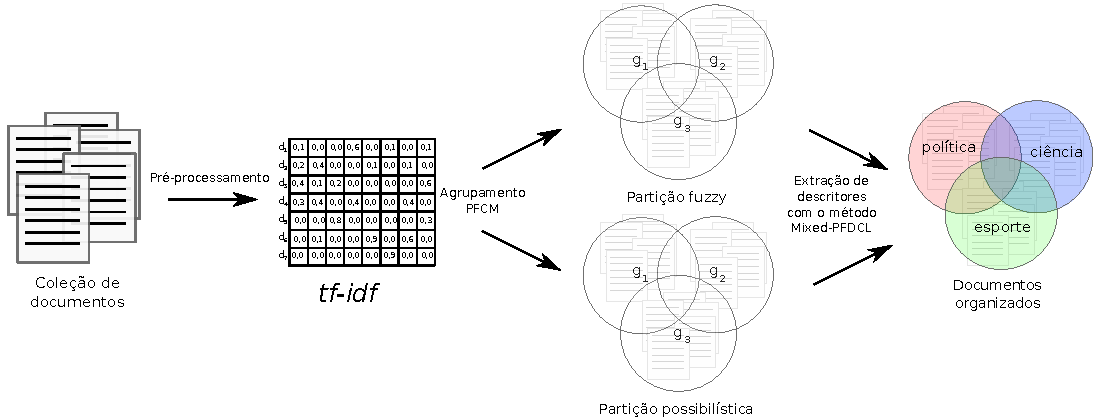
\includegraphics[width=1.0\columnwidth]{assets/process_pfdcl.pdf} 
  \caption{Estratégia híbrida proposta para uma organização flexível de documentos com o 
  agrupamento com o método PFCM e a extração de descritores com o método Mixed-PFDCL.} 
  \label{fig:pfdclprocess} 
\end{figure}


Como resultado dessa combinação é preciso adaptar as medidas de ganhos, perdas, ruídos e rejeitos,
de forma a considerar a relevância de um dado documento $d$ em relação ao limiar $\delta$, a partir
da pertinência híbrida $\mu'(d_i,g_j)$. 

Essa adaptação está então disposta nas Equações (\ref{eq:ganhos2}), (\ref{eq:perdas2}),
(\ref{eq:ruidos2}) e (\ref{eq:rejeitos2}). Ressalta-se que foi mantido no somatório de ganhos,
perdas, ruídos e rejeitos, o valor de tipicidade, devido a capacidade do mesmo em expressar a real
relação de pertinência de um documento a um grupo, devido a remoção da restrição probabilística
(Equação \ref{eq:fcmrestri1}) do
FCM. As demais medidas de precisão, recuperação e $f1$, permanecem com a mesma
definição apresentada anteriormente. Para uma melhor compreensão do método proposto, um pseudo
código do método Mixed-PFDCL está apresentado no Algoritmo \ref{alg:mixedpfdcl}.

\begin{equation}
  ganhos(t_i,g_j) = 
  \sum_{
      d \in D' 
  } \lambda(d,g_j), D' = \left\{d | d \in D, \mu'(d,g_j) \geq \delta, \varphi(t_i,d) > 0
  \right\}
  \label{eq:ganhos2}
\end{equation}
\begin{equation}
  perdas(t_i,g_j) = 
  \sum_{
      d \in D' 
  } \lambda(d,g_j), D' = \left\{d | d \in D, \mu'(d,g_j) \geq \delta, \varphi(t_i,d) = 0
  \right\}
  \label{eq:perdas2}
\end{equation}
\begin{equation}
  \text{\it ruídos\/}(t_i,g_j) = 
  \sum_{
      d \in D' 
  } \lambda(d,g_j), D' = \left\{d | d \in D, \mu'(d,g_j) < \delta, \varphi(t_i,d) > 0 \right\}
  \label{eq:ruidos2}
\end{equation}
\begin{equation}
  \text{\it rejeitos\/}(t_i,g_j) = 
  \sum_{
      d \in D' 
  } \lambda(d,g_j), D' = \left\{d | d \in D, \mu'(d,g_j) < \delta, \varphi(t_i,d) = 0 \right\}
  \label{eq:rejeitos2}
\end{equation}

\begin{algorithm}[!htp] 
  \SetAlgoLined 
  \textbf{{\color{blue}pdcl}(P, D, G, m)}\\
  \Begin{
    descritores $\gets \emptyset$\;
    \ForEach{$g \in G$}{
      candidatos $\gets [t_1,t_2,...,t_k]$\;
      ranking $\gets \emptyset$\;
      \ForEach{$t \in$ candidatos}{
        precisao $\gets$ Equação (\ref{eq:precision})\;
        recuperacao $\gets$ Equação (\ref{eq:recall})\;
        pontuacao $\gets$ Equação (\ref{eq:fmeasure})\;
        ranking[t] $\gets$ pontuacao\;
      }
      descritores[g] $\gets$ $m$ termos do ranking com maior pontuacao\;
    }
    $\textbf{retorne}$ (descritores)\; 
  }
  \caption{Pseudo código do método de extração de descritores PDCL. Onde
    considere P a partição
  possibilística (Equação \ref{eq:pcmpart}), D a coleção de documentos da coleção, G os grupos
produzidos pelo método de agrupamento e $m$ a quantidade descritores desejada por grupo.}
\label{alg:pdcl} 
\end{algorithm}

\begin{algorithm}[!htp] 
  \SetAlgoLined 
  \textbf{{\color{blue}mixed-pfdcl}(U, P, D, G, m, a, b)}\\
  \Begin{
    descritores $\gets \emptyset$\;
    \ForEach{$g \in G$}{
      candidatos $\gets [t_1,t_2,...,t_k]$\;
      ranking $\gets \emptyset$\;
      \ForEach{$t \in$ candidatos}{
        precisao $\gets$ Equação (\ref{eq:precision2})\;
        recuperacao $\gets$ Equação (\ref{eq:recall2}) \;
        pontuacao $\gets$ Equação (\ref{eq:fmeasure})\;
        ranking[t] $\gets$ pontuacao\;
      }
      descritores[g] $\gets$ $m$ termos do ranking com maior pontuacao\;
    }
    $\textbf{retorne}$ (descritores)\; 
  }
  \caption{Pseudo código do método de extração de descritores Mixed-PFDCL. Onde
    considere U a
  partição de pertinências fuzzy (Equação \ref{eq:part_fuzzy}), P a partição
  possibilística (Equação \ref{eq:pcmpart}), D a coleção de documentos da coleção, G os grupos
produzidos pelo método de agrupamento, $m$ a quantidade descritores desejada por grupo e $a,b$ os
parâmetros do PFCM.}
\label{alg:mixedpfdcl} 
\end{algorithm}

\subsection{Resultados}

Para mensurar os impactos das duas propostas (PDCL e Mixed-PFDCL) para extração de descritores apresentadas
aqui nesta seção, foi realizado outro experimento, com os algoritmos PCM e PFCM, com as bases
apresentadas na seção \ref{section:datasets}. Durante o experimento fora utilizado os métodos de
extração de descritores SoftO-FDCL, PDCL, Mixed-PFDCL. 

Uma vez que as propostas aqui apresentadas têm por objetivo otimizar os resultados apresentados
anteriormente, foi adotada uma metodologia similar aos experimentos anteriores. Ou seja, o agrupamento
final obtido para cada base, é resultado dos grupos que obtiveram o maior valor na medida de
silhueta fuzzy. Onde a quantidade de grupos para cada base, variou entre 2 e o número de classes
de cada base (Tabela \ref{table:datasets}). Ressalta-se ainda que para minimizar os efeitos da
aleatoriedade da partição inicial nesse experimento, o agrupamento foi executado 5 vezes para cada
quantidade de grupos na silhueta fuzzy. 

Os parâmetros $m$ e $n$ que regulam a variação entre fuzzy e $crisp$ das partições resultantes,
conforme ilustrados nas Figuras \ref{fig:cluster_crisp} e \ref{fig:cluster_fuzzy} foram definidos
para 1,2 de maneira empírica. De maneira geral, observou-se que as bases de maior dimensionalidade,
estavam produzindo grupos coincidentes mais facilmente, quando os valores de $m$ e $n$ eram maior do
que $1.5$. Por sua vez, os parâmetros $a$ e $b$ do algoritmo PFCM, o qual define a influência das
pertinências fuzzy do FCM e os graus de compatibilidade possibilísticos do PCM respectivamente,
foram definidos como sendo $a = 1,0$ e $b = 1,2$. Essa escolha deriva das conclusões apresentadas
em \citeonline{Pal2005}, o qual sugere que de acordo com a função objetivo (Equação
\ref{eq:pfcmobj}) do PFCM, se forem utilizados valores de $a$ maiores que $b$, os protótipos dos grupos
são mais influenciados pelas pertinências. Contudo, como em coleções textuais 
naturalmente esparsas é mais comum haver documentos ruidosos, o qual não se encaixe totalmente em
nenhum grupo, foi adotado o valor de $b$ maior do que $a$, para reduzir os efeitos
indesejados dos ruídos.

As coleções foram então agrupadas com os métodos PCM e PFCM, utilizando a metodologia descrita. A
quantidade ótima de grupos, obtida com o método da silhueta fuzzy, está apresentado na Tabela
\ref{table:pfcmclusters}. Os resultados apresentado nesta tabela, reforçam as conclusões
apresentadas experimento anterior, de que a quantidade de grupos ótima do método PFCM tende a se
aproximar mais da quantidade original de classes de cada coleção, enquanto o método PCM possui uma
tendência em obter um número de grupos bem inferior a quantidade original de classes.

\begin{table}[!htp]
  \centering
  \begin{tabular}{ |l|c|c|c|c|}
    \hline
    {\bf Coleção} & {\bf \# classes} & {\bf PCM} & {\bf PFCM} \\
    \hline
    Opinosis & 3 & 2 & 3 \\
    \hline
    20Newsgroup & 4 & 4 & 4 \\
    \hline
    Hitech & 6 & 2 & 6 \\
    \hline
    NSF & 16 &  2 & 8 \\
    \hline
    WAP & 20 & 2 & 17 \\
    \hline
    Reuters-21578 & 43 & 4 & 40 \\
    \hline
  \end{tabular}
  \caption{Quantidade ótima de grupos determinada através do método da silhueta fuzzy para cada
  algoritmo de agrupamento no segundo experimento conduzido com os métodos PCM e PFCM}
  \label{table:pfcmclusters}
\end{table}

Em seguida, foi realizado a extração dos descritores sobre as partições ótimas encontradas por
cada algoritmo de agrupamento, sobre as coleções textuais. Como a motivação desse experimento, foi
avaliar a qualidade dos descritores produzidos pelos métodos PDCL e Mixed-PFDCL propostos, a extração
de descritores foi também realizada com o método SoftO-FDCL, possibilitando assim compararmos os
resultados. E assim como no experimento anterior, essa análise quantitativa dos descritores
produzidos, foi feita, utilizando a mesma estratégia de avaliação preditiva,
com os 5 algoritmos de classificação do experimento anterior. No entanto, como a proposta de
interpretação das duas partições produzidas pelo algoritmo PFCM, contempla um grau de
compatibilidade misto entre as duas partições, foi pertinente generalizar essa interpretação
também para função de defuzificação dos grupos, apresentada na Equação
(\ref{eq:class}). Essa adaptação está apresentada na Equação (\ref{eq:class2}), onde 
foi adicionado, o grau de compatibilidade híbrido proposto na Equação (\ref{eq:pfcmmix}).

\begin{equation}
  crisp(d_i) = \begin{cases}
    crisp_j, & \mu(d_i,g_j) = \displaystyle\max_{\forall g \in G} \mu(d_i,g), \text{se a partição
  for fuzzy}\\
  crisp_j, & \lambda(d_i,g_j) = \displaystyle\max_{\forall g \in G} \lambda(d_i,g), \text{se a
  partição for possibilística}\\
  crisp_j, & \mu'(d_i,g_j) = \displaystyle\max_{\forall g \in G} \mu'(d_i,g), \text{se houver
duas partições}
  \end{cases}
  \label{eq:class2}
\end{equation}

Sendo assim, é realizada uma redução na matrix documentos x termos original para a matriz documentos
x descritores, conforme descrito na seção \ref{sec:exppfcm}, onde a pertinência de cada documento é
submetida a uma defuzificação com a Equação (\ref{eq:class2}). Posteriormente, essa matriz de
dimensionalidade reduzida é submetida aos mesmos classificadores do experimento anterior, com os
mesmos parâmetros. Os resultados dessa classificação estão apresentados nas Figuras
\ref{fig:pdclopinosis}, \ref{fig:pdcl20news}, \ref{fig:pdclhitech}, \ref{fig:pdclnsf},
\ref{fig:pdclwap} e \ref{fig:pdclreuters}.

\begin{figure}[!h] \centering 
   \begin{minipage}{0.48\textwidth} 
     \centering
    \includegraphics[width=1.0\columnwidth]{assets/pdcl/opinosis} 
    \caption{Desempenho obtido dos descritores extraídos com os algoritmos SoftO-FDCL, Mixed-PFDCL e
    PDCL sobre o agrupamento produzido pelos métodos PCM e PFCM na coleção Opinosis} 
  \label{fig:pdclopinosis}
  \end{minipage}\hfill 
  \begin{minipage}{0.48\textwidth} \centering
    \includegraphics[width=1.0\columnwidth]{assets/pdcl/newsgroup} 
    \caption{Desempenho obtido dos descritores extraídos com os algoritmos SoftO-FDCL, Mixed-PFDCL e
    PDCL sobre o agrupamento produzido pelos métodos PCM e PFCM na coleção 20Newsgroup} 
     \label{fig:pdcl20news} 
   \end{minipage} 
\end{figure}

\begin{figure}[!h] \centering 
   \begin{minipage}{0.48\textwidth} 
     \centering
    \includegraphics[width=1.0\columnwidth]{assets/pdcl/hitech} 
    \caption{Desempenho obtido dos descritores extraídos com os algoritmos SoftO-FDCL, Mixed-PFDCL e
    PDCL sobre o agrupamento produzido pelos métodos PCM e PFCM na coleção Hitech} 
  \label{fig:pdclhitech}
  \end{minipage}\hfill 
  \begin{minipage}{0.48\textwidth} \centering
    \includegraphics[width=1.0\columnwidth]{assets/pdcl/nsf} 
    \caption{Desempenho obtido dos descritores extraídos com os algoritmos SoftO-FDCL, Mixed-PFDCL e
    PDCL sobre o agrupamento produzido pelos métodos PCM e PFCM na coleção NSF} 
     \label{fig:pdclnsf} 
   \end{minipage} 
\end{figure}

\begin{figure}[!h] \centering 
   \begin{minipage}{0.48\textwidth} 
     \centering
    \includegraphics[width=1.0\columnwidth]{assets/pdcl/wap} 
    \caption{Desempenho obtido dos descritores extraídos com os algoritmos SoftO-FDCL, Mixed-PFDCL e
    PDCL sobre o agrupamento produzido pelos métodos PCM e PFCM na coleção WAP} 
    \label{fig:pdclwap}
  \end{minipage}\hfill 
  \begin{minipage}{0.48\textwidth} \centering
    \includegraphics[width=1.0\columnwidth]{assets/pdcl/reuters} 
    \caption{Desempenho obtido dos descritores extraídos com os algoritmos SoftO-FDCL, Mixed-PFDCL e
    PDCL sobre o agrupamento produzido pelos métodos PCM e PFCM na coleção Reuters-21578} 
     \label{fig:pdclreuters} 
   \end{minipage} 
\end{figure}

O sumário desses resultados consta na Tabela \ref{table:pdclsummary}, onde o marcador ($\checkmark$)
denota que o método obteve maiores taxas de acerto entre os 5 algoritmos de classificação
utilizados. Como nessa investigação o propósito foi comparar os métodos de extração de descritores,
dividiu-se o sumário de resultados de acordo com o método de agrupamento, PCM e PFCM
respectivamente. Ressalta-se ainda, que garantir que a extração fosse realizada sobre os mesmos
grupos, ambos os
métodos de extração de descritores foram aplicados simultaneamente ao agrupamento. Portanto, os
métodos SoftO-FDCL e PDCL foram aplicados ao mesmo agrupamento produzido pelo PCM, enquanto o
SoftO-FDCL e o Mixed-PFDCL foram executados no mesmo agrupamento gerado pelo PFCM. 

Os resultados dispostos nesse sumário, corroboram a hipótese formulada a respeito da interpretação
das partições possibilísticas e híbridas no contexto da extração de descritores para a organização
flexível de documentos. Pois, como se observa na Tabela \ref{table:pdclsummary}, o método PDCL e o
Mixed-PFDCL, superam os resultados do método SoftO-FDCL, em ambos os algoritmos de agrupamento.
Embora, tenha existido 2 empates na comparação entre os métodos SoftO-FDCL e PDCL, para as coleções
20newsgroups e NSF.

\begin{table}[!htp]
  \centering
  \begin{tabular}{|l|c c|c c|}
    \hline
    & \multicolumn{2}{c|}{PCM} & \multicolumn{2}{c|}{PFCM} \\
    \hline
    {\bf Coleção} & SoftO-FDCL & PDCL & SoftO-FDCL & Mixed-PFDCL \\
    \hline
    {\bf Opinosis} & & $\checkmark$ & & $\checkmark$ \\
    \hline
    {\bf 20newsgroups} & $\checkmark$ & $\checkmark$ & & $\checkmark$\\
    \hline
    {\bf Hitech} & & $\checkmark$ & & $\checkmark$ \\
    \hline
    {\bf NSF} &  $\checkmark$ & $\checkmark$ & & $\checkmark$\\
    \hline
    {\bf WAP} & & $\checkmark$ & & $\checkmark$\\
    \hline
    {\bf Reuters-21578} & & $\checkmark$ & & $\checkmark$\\
    \hline
  \end{tabular}
  \caption{Sumário dos resultados da classificação dos descritores extraídos com os métodos
  SoftO-FDCL, PDCL e Mixed-PFDCL}
  \label{table:pdclsummary}
\end{table}

Ao se analisar os resultados, comparando as taxas de acerto obtidas entre os métodos de agrupamento,
é possível se observar uma relevante tendência do PCM superar o PFCM. Entretanto, as taxas de acerto
próximas de 100\% no PCM, desperta atenção. Nesse sentido, vamos analisar na Tabela
\ref{table:pdclmajority}, os grupos majoritários da matriz documentos x descritores, obtidos após a
defuzificação do agrupamento com a Equação (\ref{eq:class2}), para entender o por que de taxas tão
elevadas. 

\begin{table}[!htp]
  \centering
  \begin{tabular}{|l|c|c c|}
    \hline
    & PCM & \multicolumn{2}{c|}{PFCM} \\
    \hline
    {\bf Coleção} & SoftO-FDCL e PDCL & SoftO-FDCL & Mixed-PFDCL \\
    \hline
    {\bf Opinosis} & 84,31\% & 43,13\% & 43,13\% \\
    \hline
    {\bf 20newsgroups} & 99,9\% & 49,55\% & 51,65\% \\
    \hline
    {\bf Hitech} & 95,16\% & 25,83\% & 25,83\% \\
    \hline
    {\bf NSF} & 100\% & 44,43\% &  34,21\% \\
    \hline
    {\bf WAP} & 93,3\% & 57,69\% & 86,53\% \\
    \hline
    {\bf Reuters-21578} & 97,81\% & 68,91\% & 76,42\% \\
    \hline
  \end{tabular}
  \caption{Informações das classes majoritárias obtidas através da defuzificação dos grupos fuzzy,
  com a Equação (\ref{eq:class2})}
  \label{table:pdclmajority}
\end{table}

É demonstrado então na Tabela \ref{table:pdclmajority}, que a defuzificação dos agrupamentos
produzidos pelo método PCM em cada coleção, resultou em grupos majoritários próximo de 100\%, o que
por sua vez facilita a tarefa do classificador. Desse modo, fica claro as causas de taxas de acertos
tão elevadas no método PCM, e assim como também nos mostra a importância de não analisarmos os
resultados da classificação isoladamente. Por outro lado, percebe-se na Tabela
\ref{table:pdclmajority}, a discrepância dos grupos majoritários no algoritmo PFCM em comparação ao
PCM. Isso por sua vez, indica que o agrupamento produzido pelo PFCM, gerou grupos mais coerentes, o
que reforça a adequação desse algoritmo para coleções textuais.

Nos estudos do limiar $\delta$, detalhados na seção \ref{sec:softofdcl}, foi pontuado que ao 
se utilizar esse limiar em partições possibilísticas, poderia resultar em listas similares de
descritores entre os grupos. Portanto, para comprovar essas conclusões obtidas dessa
investigação, é pertinente analisar as listas dos descritores com maior pontuação em cada grupo,
produzidas pelos métodos Soft-FDCL, PDCL e Mixed-PFDCL nesse experimento. Contudo, como são muitas
bases, e em alguns casos a quantidade de grupos é demasiadamente elevada, está apresentado nas
Tabelas \ref{table:rankingpdcl} e \ref{table:rankingmixedpdcl}, somente as 5 maiores pontuações dos
termos candidatos aos grupos obtidos pelos algoritmos PCM e PFCM na base Opinosis. Assim como no
experimento anterior, foi escolhido apresentar essa base, para facilitar a interpretação dos
resultados, pois a mesma contém uma quantidade baixa de documentos e de grupos resultantes do
agrupamento.

\begin{table}[!htp]
  \centering
  \begin{tabular}{ |l| l l | l l|}
    \hline
    & \multicolumn{2}{c|}{$grupo_1$} & \multicolumn{2}{c|}{$grupo_2$} \\
    \hline
    {\bf método} & termo & pontuação & termo & pontuação \\
    \hline
    \multirow{5}{*}{{\bf SoftO-FDCL}} & caf & 0,923077 & caf & 0,923077 \\
                                       & floor	    & 0.888889  & floor	  & 0.888889 \\
                                       & food	    & 0.880000  & food	  & 0.880000 \\
                                       & coffe	    & 0.857143  & coffe	  & 0.857143 \\
                                       & concierge  & 0.846154  & concierge & 0.846154 \\
    \hline
    \multirow{5}{*}{{\bf PDCL}} & bathro      &  0.894716  & make    & 0.800980 \\       
                                 & food        &  0.888785  & time    & 0.789846 \\       
                                 & concierge    &  0.860127  & nice    & 0.779338 \\       
                                 & supermarket &  0.856632  & feature & 0.778138 \\       
                                 & chain       &  0.856632  & easy    & 0.768564 \\       
    \hline
  \end{tabular}
  \caption{Lista ordenada com 5 termos candidatos de maior pontuação, obtidos após a extração de
  descritores com os métodos Soft-FDCL e PDCL aplicados ao agrupamento da coleção Opinosis com o
algoritmo PCM}
  \label{table:rankingpdcl}
\end{table}

Portanto, ao se analisar na Tabela \ref{table:rankingpdcl}, as pontuações e os termos do $grupo_1$ e
do $grupo_2$, obtidos com o método SoftO-FDCL, nota-se uma repetição dos termos e pontuações para
ambos os grupos. Essa evidência, por usa vez, fortalece a problemática na interpretação dos graus de
compatibilidade possibilísticos apresentada na seção \ref{sec:softofdcl}.  Por outro lado, os termos
obtidos com o método proposto, não se repetem em ambos os grupos, assim como também estão mais
coerentes entre si. Conforme foi detalhado, a base Opinosis é composta de uma série de opiniões
sobre eletrônicos, hotéis e carros, sendo assim é possível observar nos termos encontrados pelo
método PDCL, uma proximidade semântica com esses assuntos.

Já Tabela \ref{table:rankingmixedpdcl}, a qual contém os 5 termos candidatos de maior pontuação no 
$grupo_1$, $grupo_2$ e $grupo_3$, não apresentou o problema da repetição dos mesmos termos nos
grupos para o método SoftO-FDCL. Isto se deve por conta da extração de descritores com o método
SoftO-FDCL nesse experimento, utilizar somente os graus de pertinências, os são adequados a este
método, conforme foi destacado durante a investigação desse método. Contudo, no experimento
anterior, foi levantado a importância de se utilizar as pertinências e tipicidades presentes no
algoritmo PFCM, para melhor interpretar o agrupamento produzido por essa abordagem híbrida. Nesse
contexto, observa-se que os termos de maior pontuação do método Mixed-PFDCL, diferem parcialmente
dos termos obtidos com o método SoftO-FDCL, porém há de se observar que os termos dos grupos
SoftO-FDCL podem ser semanticamente relacionados aos termos do método Mixed-PFDCL. Ainda é possível
notar, que os 3 grupos de termos são similares aos 3 tópicos presentes na coleção Opinosis. O que
por sua vez, reforça a adequadação do método proposto para interpretar de maneira híbrida ambas as
partições geradas no pelo método PFCM.

\begin{table}[!h]
  \centering
  \begin{tabular}{ | l | l l | l l | l l |}
    \hline
    & \multicolumn{2}{c|}{$grupo_1$} & \multicolumn{2}{c|}{$grupo_2$} &
    \multicolumn{2}{c|}{$grupo_3$} \\
    \hline
    {\bf método} & termo & pontuação & termo & pontuação & termo & pontuação \\
    \hline
 \multirow{5}{*}{{\bf SoftO-FDCL}} & text   & 0.850000 & coffe  &  0.933333 &  ga     & 0.833333 \\
                                    & featur & 0.758621 & eat   &  0.903226 &  camr   & 0.818182 \\
                                    & device  & 0.750000 & floor   &  0.896552 &  transmission & 0.818182 \\
                                    & user   & 0.750000 & inn   &  0.896552 &  seat   & 0.769231 \\
                                    & unit   & 0.727273 & lobby  &  0.896552 &  rir    & 0.769231 \\
    \hline
 \multirow{5}{*}{{\bf Mixed-PFDCL}} & featur & 0.876540 & friendl & 0.951225 & fun & 0.891245  \\
&  text          &  0.869230  &  bed           &  0.950665  &  ga            &  0.868032  \\
&  find          &  0.830332  &  coffe          &  0.948341  &  rir           &  0.847864  \\
&  isnt           &  0.817311  &  stay           &  0.945294  &  seat          &  0.843576  \\
&  easy           &  0.809918  &  night         &  0.933519  &  engine         &  0.840700  \\
    \hline
  \end{tabular}
  \caption{Lista ordenada com 5 termos candidatos de maior pontuação, obtidos após a extração de
  descritores com os métodos Soft-FDCL e PDCL aplicados ao agrupamento da coleção Opinosis com o
algoritmo PFCM}
  \label{table:rankingmixedpdcl}
\end{table}

Na próxima seção será apresentado uma breve sintése dos experimentos conduzidos nesse capítulo,
pontuando as principais contribuições e descobertas encontradas ao longo desse processo de
investigação.

\section{Considerações finais}

Neste capítulo foi detalhado todo o processo de investigação realizado nessa monografia, assim como
a metodologia utilizada para a realização dos experimentos, informações das coleções textuais
utilizadas e as devidas análises dos resultados. A abordagem híbrida proposta por essa monografia
constitui a adição da robustez proporcionada pelo algoritmo PFCM o qual é uma versão híbrida dos
algoritmos FCM e PCM. Durante esse processo, foi identificado no primeiro experimento, que era
preciso propor uma maneira de melhor interpretar as tipicidades do algoritmo PCM. Outra conclusão
obtida do primeiro experimento, foi também a necessidade de realizar a extração de descritores dos
grupos produzidos pelo método PFCM utilizando as duas partições. Nesse sentido, foi aqui
apresentada uma abordagem para corretamente se interpretar as tipicidades, assim como também uma
estratégia híbrida para se realizar a extração de descritores do método PFCM.

No próximo capítulo, será abordada as conclusões a respeito de toda a pesquisa apresentada nessa
monografia.


